\chapter{Wireless Interface}

Four methods of a wireless connection have been considered: Bluetooth (e.g. with CC2541), WiFi with ESP8266, LoRA or GFSK-modulated 868\,MHz link with SX1276, and a 2.4\,GHz link with nRF24L01+. Bluetooth was dismissed early for its complexity and ESP8266 for its high consumption in continuous reception mode, although both solutions might be viable for certain applications and with more time for evaluation. 

The Semtech SX1276 and Nordic Semiconductor nRF24L01+ transceivers have both been tested using the first GEX prototype, confirming its usefulness as a hardware development tool, and it's been confirmed they could fulfill the requirements of the application.

\begin{figure}[h]
	\centering
	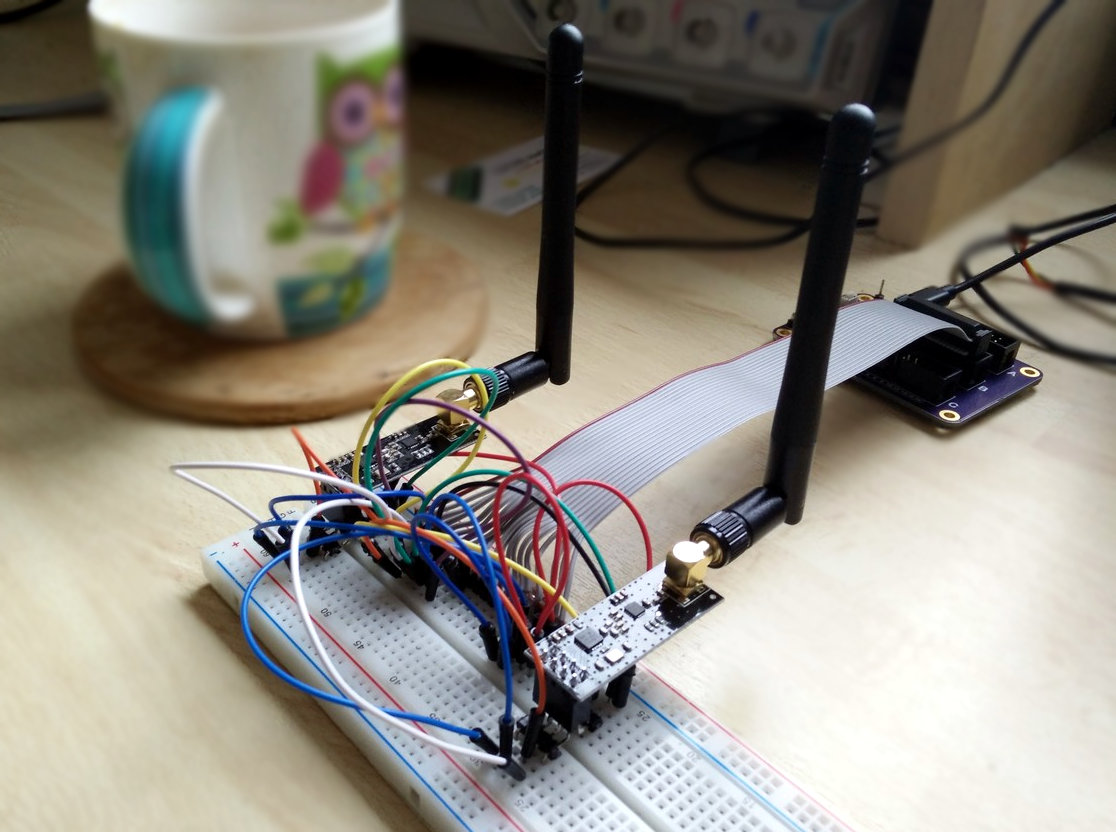
\includegraphics[width=.7\textwidth]{img/nrf-testing.jpg}
	\caption{Test setup with a GEX prototype controlling two nRF24L01+ modules}
\end{figure}


\section{Comparing SX1276 vs. nRF24L01+}

The two transceivers are compared in table \ref{fig:nrf-sx-comparison}. It's apparent that each has its strengths and weaknesses.

\begin{table}[h]
	\centering
	\begin{tabulary}{\textwidth}{lLL}
		\toprule
		\textbf{Parameter} & \textbf{SX1276} & \textbf{nRF24L01+} \\
		\midrule
		\textbf{Connection} & SPI (4 pins) + up to 6 IRQ & SPI (4 pins), CE, IRQ \\
		\textbf{Frequency band} & 868\,MHz or 433\,MHz & 2.4\,GHz \\
		\textbf{Data rate} & up to 300\,kbps & 250--2000\,kbps \\
		\textbf{Modulation} & (G)FSK, (G)MSK, OOK, LoRa & GFSK \\
		%		\textbf{Bandwidth} & 7--500\,kHz per channel & 0.7--2\,MHz per channel \\
		\textbf{Range (est.)} & 2\,km to 20\,km LOS & up to 1\,km LOS \\
		\textbf{Consumption Rx} & 10.8--12\,mA & 12.6--13.5\,mA \\
		\textbf{Consumption Tx} & 20--120\,mA & 7--11.3\,mA \\
		\textbf{Idle power (max)} & 1\,$\mu$A sleep, 2\,mA stand-by & 0.9\,$\mu$A sleep, 320\,$\mu$A stand-by \\
		\textbf{Max packet size} & 300 bytes & 32 bytes \\
		\textbf{Reset} & NRESET pin & Vdd disconnect \\
		\textbf{Extra} & LoRa FHSS, packet engine & ShockBurst protocol engine \\
		\textbf{Price} & \$7.3 & \$1.6 \\
		\bottomrule
	\end{tabulary}
	\caption[Comparison of the SX1276 and nRF24L01+ wireless transceivers]{\label{fig:nrf-sx-comparison}Comparison of the SX1276 and nRF24L01+ wireless transceivers (price from DigiKey @ 10 pieces, May 6th 2018)}
\end{table}

SX1276 supports additional modulation modes, including a proprietary LoRa scheme with a frequency-hopping spread spectrum modulation that can be received at a distance up to 20\,km in ideal conditions. The long-range capability is reflected in a higher consumption during transmission. However, its consumption in receiver mode is slightly lower than that of the nRF24L01+.

nRF24L01+ provides higher data rates at short distances. Its power consumption is comparable or lower than that of the SX1276. It lacks a dedicated reset pin, but that can be easily worked around using an external transistor to momentarily disconnect its Vdd pin.

Both devices implement some form of a packet engine with error checking; that of the nRF24L01+, called ShockBurst, is more advanced as it implements acknowledgment responses and automatic re-transmission, leading to a potentially more robust communication without an additional overhead on the side of the microcontroller. 


\section{Integration of the nRF24L01+ into GEX}

The nRF24L01+ was selected to be integrated into GEX thanks to its inclusion of the ShockBurst engine, higher possible data rates and significantly lower price. The SX1276, nonetheless, remains an interesting option that could be used as an alternative in the future, should the need for a long range communication arise.

A separate device, the \textit{GEX wireless gateway}, was developed to provide the PC connection to a nRF24L01+ module. It is based on the STM32F103 microcontroller in its smallest package (LQFP48), selected for it's low cost and good availability.

\subsection{The Wireless Gateway Protocol}

\begin{wrapfigure}[17]{r}{0.38\textwidth}
	\vspace{-1em}
	\centering
	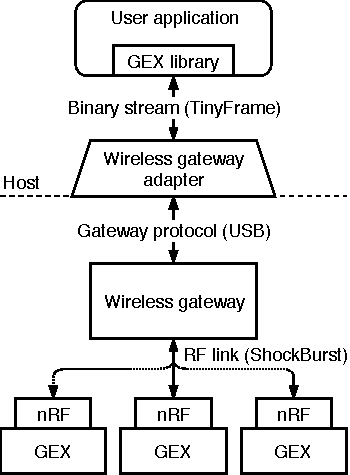
\includegraphics[scale=0.9]{img/rf-gw.pdf}
	\caption{A block diagram of the wireless connection}
\end{wrapfigure}

The gateway presents itself to the host as a CDC/ACM device, much like the GEX modules themselves (here called \textit{nodes}) when connected over USB. It implements a simple protocol which encapsulates the binary data sent to or from a connected node. The wrapped GEX protocol (chapter \ref{sec:tinyframe}) remains unchanged.

The gateway has a 4-byte network ID, a number derived from the microcontroller's unique ID. The network ID must be entered into all nodes that wish to communicate with it. Additionally, each module must be assigned a unique 1-byte number, which, together with the four network ID bytes, uniquely identifies the node. The gateway can connect to up to 6 nodes at once.

All messages sent to or from the gateway are a multiple of 64 bytes long, padded with zeros if shorter. The message starts with a control byte, determining the message type (table \ref{fig:rf-dongle-commands}).

\begin{table}[h]
	\centering
	\begin{tabulary}{\textwidth}{lL}
		\toprule
		\textbf{Function} & \textbf{Message structure} \\
		\midrule
		Send a message & 'm' (\verb|u8|)address (\verb|u16|)length (\verb|u8[]|)payload \\
		Restart \& remove nodes &  'r' \\
		Add nodes &  'n' (\verb|u8|)count (\verb|u8[]|)addresses \\
		Get the network ID &  'i' \\
		Response to 'i' & 0x01 (\verb|u8[4]|)net\_id \\
		Received message & 0x02 (\verb|u8|)address (\verb|u8|)length (\verb|u8[]|)data \\
		\bottomrule
	\end{tabulary}
	\caption[Wireless gateway commands and messages]{\label{fig:rf-dongle-commands}Wireless gateway commands and messages; control characters in the printable range are shown as ASCII}
\end{table}

The gateway may be restarted using the 'r' command when the PC application starts. Then it adds all node addresses with the 'n' command and can begin communication. The 'i' command, reading the network ID, can additionally be used as a ping command to verify the USB connection.

\todo[inline]{Add additional commands. Also remove magic bytes form the real messages, they're useless}






























